\documentclass[
	%a4paper, % Use A4 paper size
	letterpaper, % Use US letter paper size
]{jdf}

\addbibresource{references.bib}

\author{Shashvat Sinha}
\email{shashvat.sinha@gatech.edu}
\title{Project (Summer 2020)\\CS6750}

\begin{document}
%\lsstyle

\maketitle

\section{Introduction}
\subsection{Interface Description}
The interface we have chosen to redesign is the on-screen keyboard for Xbox One consoles. This interface shows up whenever a user has to type in characters from a keyboard into a textbox. It is used for searching, username and password input and the Xbox Live short message service. The keyboard made its appearance with the release of the Xbox One in November 2013.

\begin{figure}[h]
	\centering
	\frame{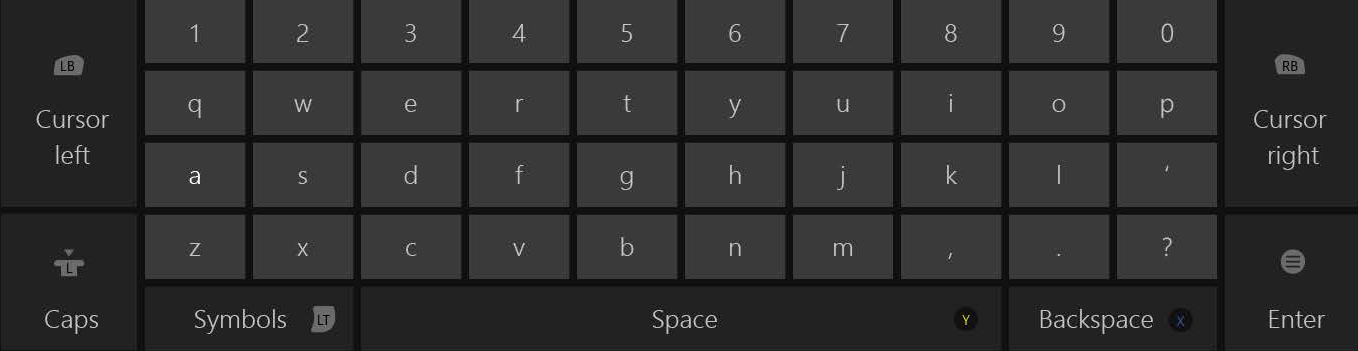
\includegraphics[width=9cm]{jdf-master/Figures/xbox-one-virtual-keyboard.jpg}}
	\caption{Xbox One Virtual Keyboard}
	\label{fig:xb1keyboard}
\end{figure}


A detailed description of the keyboard design is given on the portfolio page of the designer, Matthew Hartman (\cite{hartman_2013}).


In order to use the keyboard, one must have an Xbox One console. On the console, navigate to any screen that requires textual input, for example the search box on the Microsoft Store page, or the password input page on the wireless network configuration screen. This should bring up the keyboard on screen.

\begin{figure}[h]
	\centering
	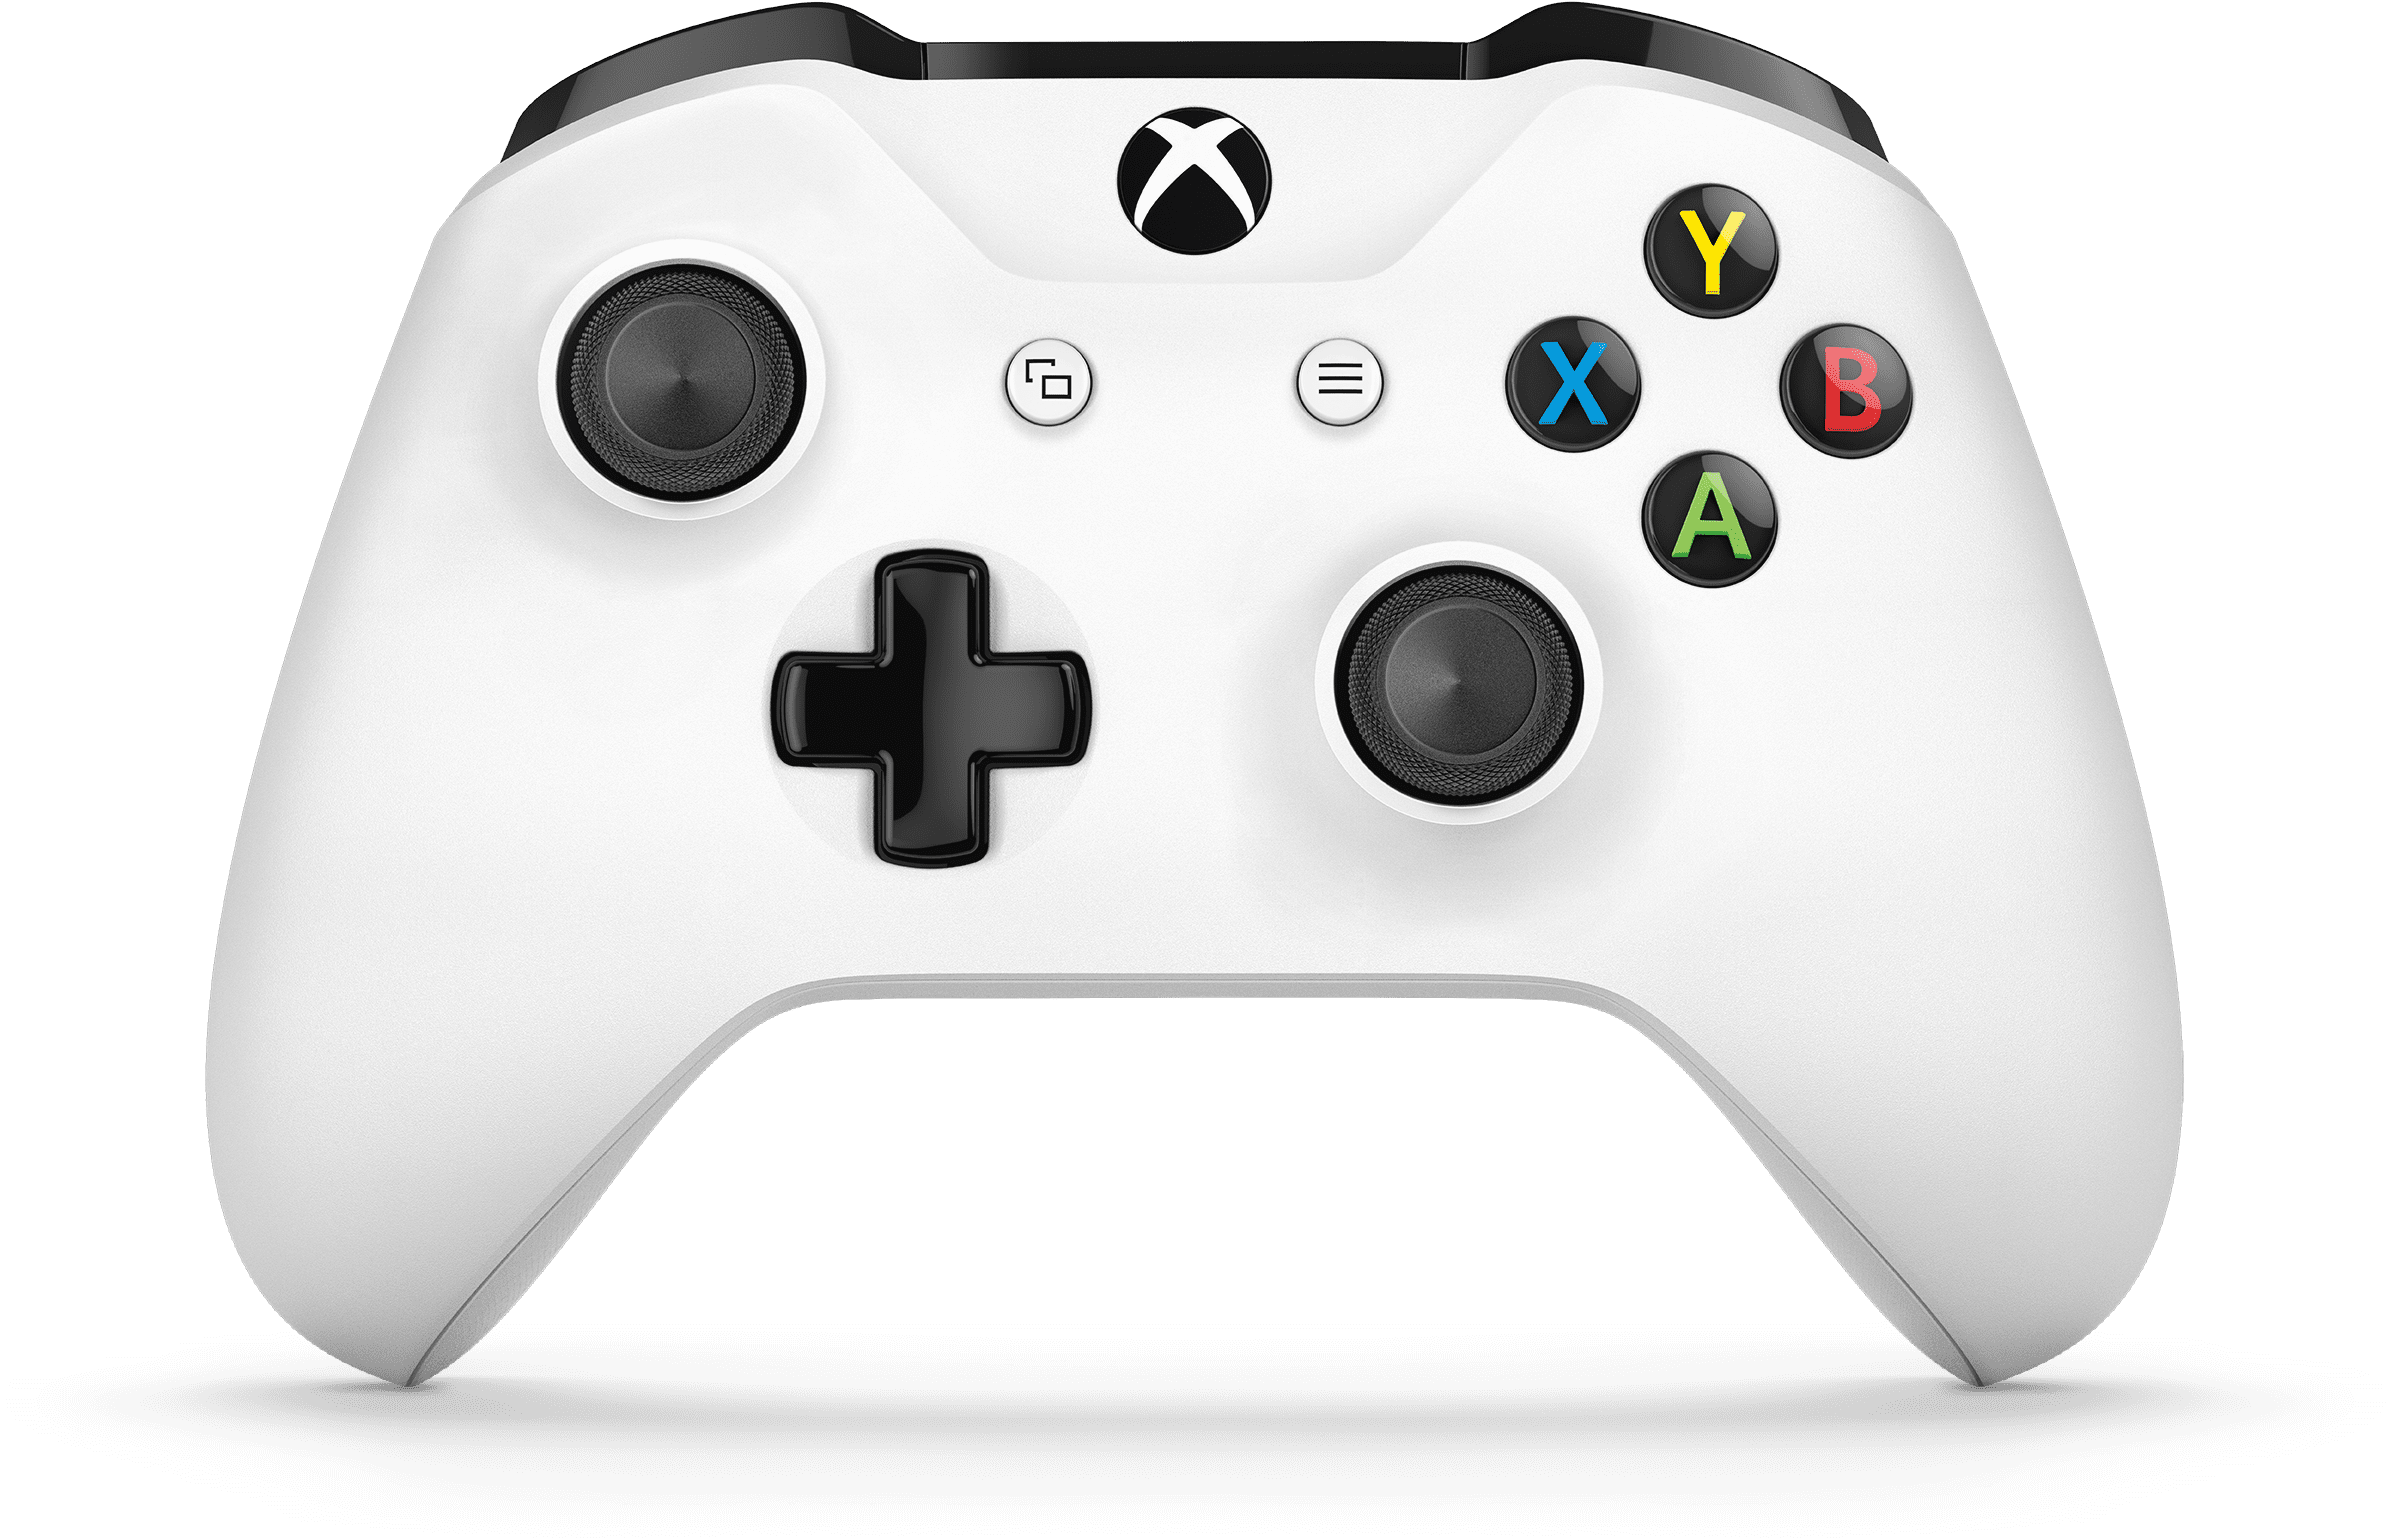
\includegraphics[width=6cm]{jdf-master/Figures/xbox-one-controller.png}
	\caption{Xbox One Controller}
	\label{fig:xb1controller}
\end{figure}

The keyboard is operated by the Xbox controller, a handheld device that has a variety of physical inputs on it - two sticks that can be moved in circular directions (thumbsticks), four colored buttons A, B, X \& Y, four directional buttons (cursor keypad), two buttons under the left and right trigger fingers (left and right triggers) and two buttons above the triggers (left and right shoulder buttons). The controller is also equipped with haptic feedback for the triggers and also general vibration. And last but not the least, the thumbsticks are also buttons, operated by pressing them axially.

The keyboard is operated by utilizing the Xbox controller to select letters to be typed, then pressing a button to select that letter. This is done one letter at a time.

\subsection{Scope}
We will not be redesigning the controller. We will only be redesigning the onscreen virtual keyboard, and the interaction of the controller with the virtual keyboard.

\section{Initial Needfinding}
\subsection{Choice of Needfinding Type}
For our initial needfinding, we will use publicly available data in the form of product reviews, opinion pages, design patents (wherein they identify particular problems they are trying to solve), scholarly papers and so on.

Our objective is to determine what are the shortcomings with the existing virtual keyboard interface on-screen of the Xbox One. 

\subsection{Needfinding Approach}
The volume of literature on the Xbox virtual QWERTY keyboard is not large by any means. So we will divide our needfinding into two parts:
\begin{itemize}
    \item Research on QWERTY keyboards, focusing on virtual/on-screen implementations.
    \item Research on game controllers input/selection techniques.
\end{itemize}

We will use Google Scholar (\url{https://scholar.google.com}) to find articles of interest. We will also use generic searches on Google search to find articles of interest.

In those articles we will search for critiques of QWERTY keyboards, find any quantitative or emperical studies performed and the results thereof.

We will also review papers and articles on methods of input using game controllers that can inform us on better approaches towards using the Xbox One Game controller for input.

\subsection{Needfinding Execution}
\subsubsection{Findings on QWERTY Keyboards}
The QWERTY keyboard was designed during the second half of the 19th century by Sholes et. al (\cite{sholes_glidden_soule_1868}) as a means of writing by type. The primiary consideration during its design was the ability of the rudimentary mechanical devices of those days to be able to function properly with the demands of typing in the English language i.e. not get jammed. There is however, a secondary reason for the layout of the keyboard in the QWERTY form, and not ABCDE form, and that was to do with the needs of the original users of the typewriter - telegraph operators (\cite{stamp_2013}), who needed a device that was well suited to transcribing Morse Code into English. It can be seen that Sholes et. al. did actually follow needfinding approaches for their HMI (human-machine-interface) product development and listened to the needs of their users, contrary to popular belief. This section of research was established the original design context of the QWERTY keyboard. That context does not exist now, and needs to be updated.

Multiple forms of research have been performed on QWERTY keyboards with critical analysis done and alternatives proposed - 

In "\textit{The design and evaluation of a high-performance soft keyboard}" (\cite{mackenzie_zhang_1999}) we see that QWERTY as a keyboard layout lags in performance when compared to other virtual keyboard types. Mackenzie and Zhang employ Fitts's Law to quantitatively model an ideal keyboard layout, which they called Opti, that had a 35\% better performance than the standard QWERTY layout - in a virtual keyboard setting.

In "\textit{Performance Optimization of Virtual Keyboards}" (\cite{zhai_hunter_smith_2002}) we see that an optimally designed Hooke keyboard has 48\% improvement in words per minute (wpm) efficiency over QWERTY while the further optimized Metropolis approach gets to 42.5 wpm movement efficiency, which was 50\% higher than Qwerty and 10\% higher than OPTI.

In \textit{"Efficient keyboard layouts for sequential access in augmentative and alternative communication"} (\cite{venkatagiri_1999}) we see that rowscanning for QWERTY keyboard layouts is far more inefficient than row-column scanning, i.e. even within QWERTY approaches, there are possibilities for optimisation.

\subsubsection{Findings on Game Controller Input}
Our objective here is to see how thumbsticks can be best employed for user input.

In \textit{"TwoStick: Writing with a Game Controller"} (\cite{twostick_2007}) we see a method for typing that uses the standard QWERTY keyboard but utilizes both thumbsticks rather than just one, for improved speed and accuracy.

\begin{figure}[h]
	\centering
	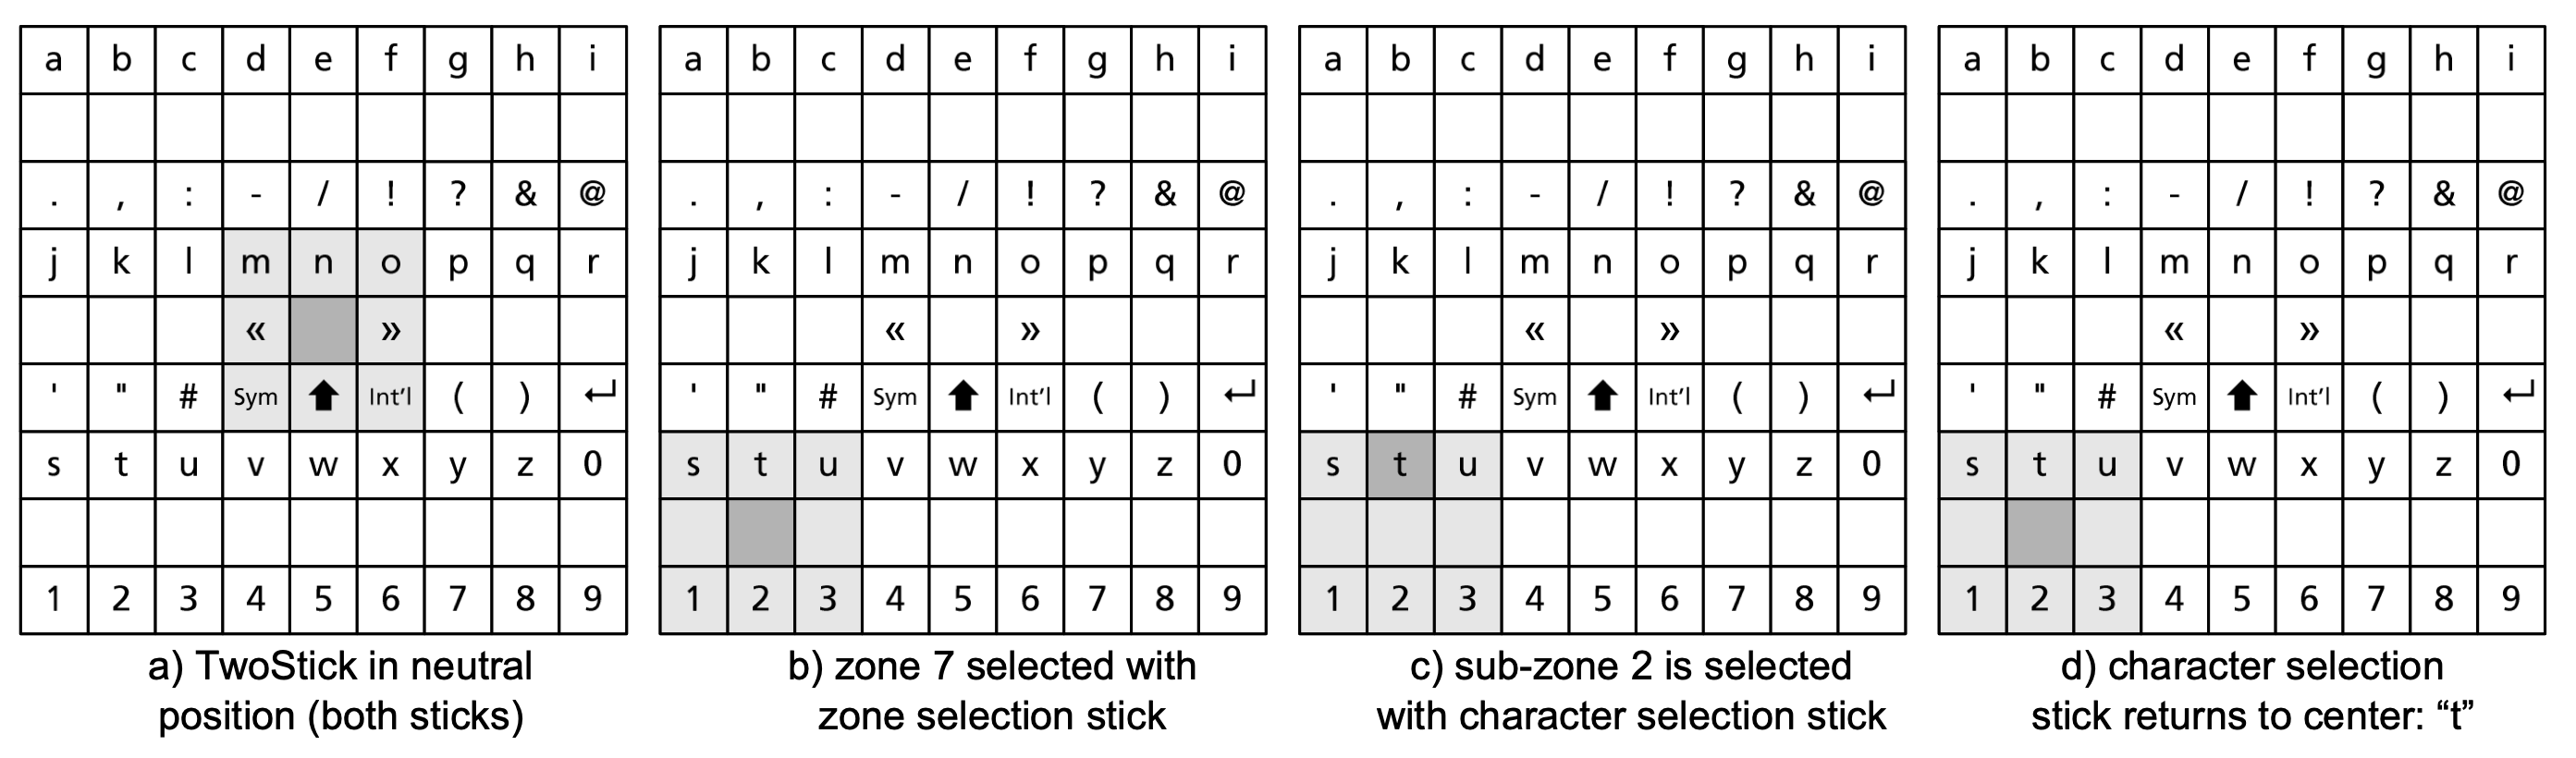
\includegraphics[width=9cm]{jdf-master/Figures/twostick.png}
	\caption{TwoStick Text Entry}
	\label{fig:twostick}
\end{figure}

In \textit{"Text Entry Using a Dual Joystick Game Controller"} (\cite{wilson_agrawala_2006}) the authors employ a dual-QWERTY layout with the left thumbstick selecting letters on the left side of an onscreen QWERTY keyboard and the right thumbstick selecting from the right. Here they saw a statistically significant difference between single-stick and double-stick input.

The patent \textit{"Graphic user interface for a digital content delivery system using circular menus"} \cite{eatsy_taplin_chechik_nelson_2002}) shows how a circular layout can be used to select menu items. 

\begin{figure}[h]
	\centering
	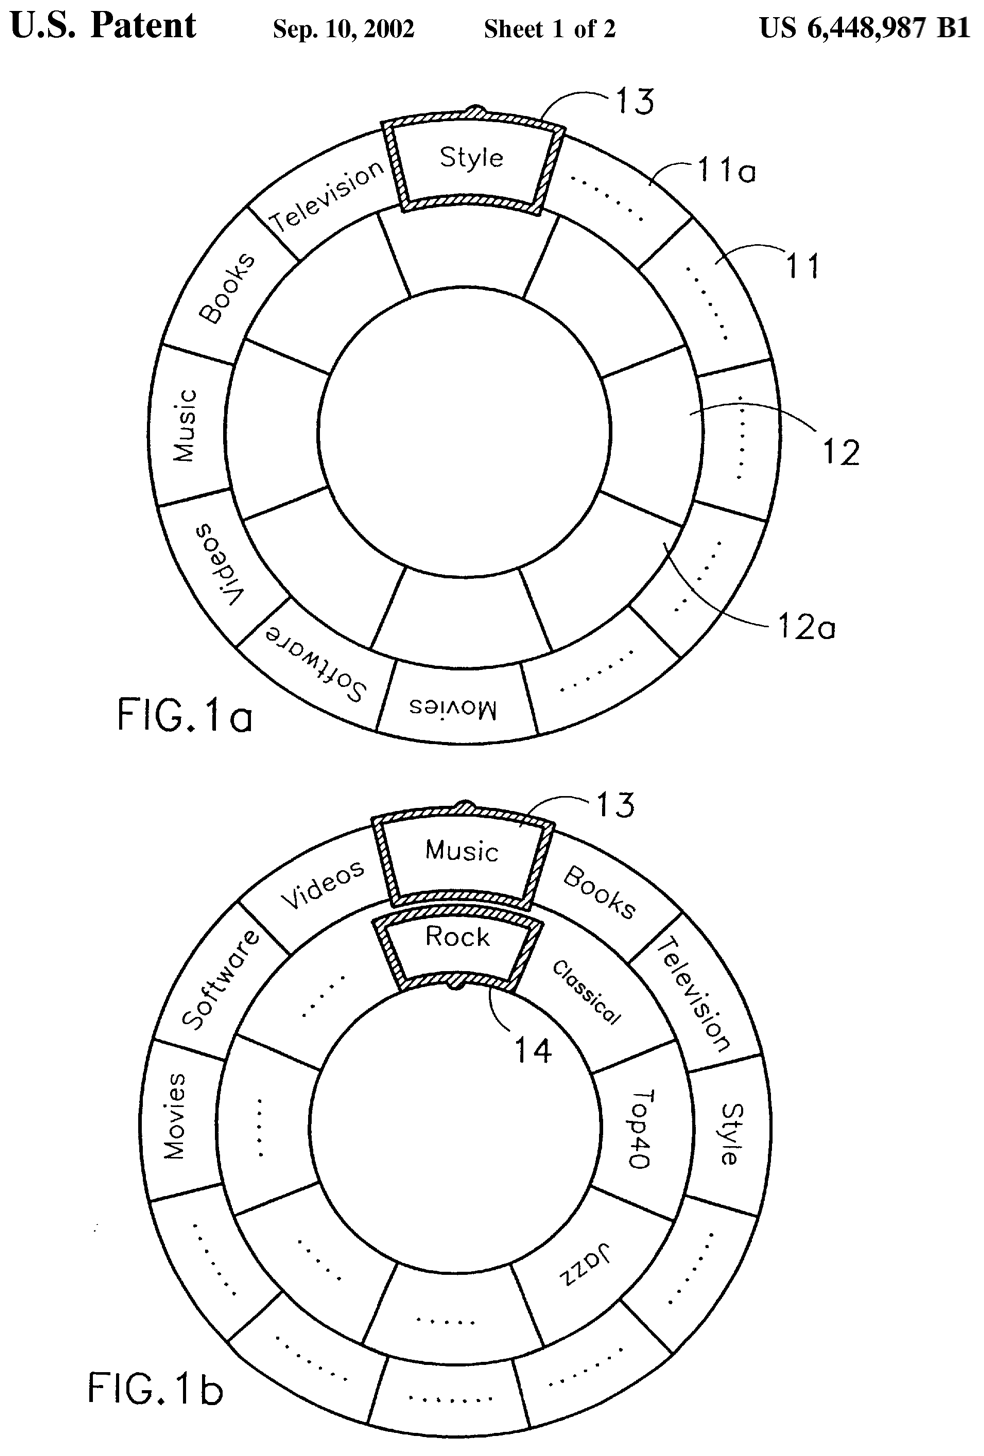
\includegraphics[width=5cm]{jdf-master/Figures/circularmenu.png}
	\caption{Circular Menus}
	\label{fig:circularmanu}
\end{figure}

\subsubsection{Conclusions}
We would make the following three conclusions from our research:
\begin{enumerate}
    \item The QWERTY keyboard layout has had sufficient research done on it to demonstrate that alternative approaches are better. However despite that, the QWERTY layout continues to be the preferred layout.
    \item Even when restricting ourselves to QWERTY layouts, it is possible to improve text input speed and accuracy by using both thumbsticks as inputs, when compared to using a single thumbstick or cursor.
    \item Thumsticks rotate in the circular domain and therefore lend themselves better to a circular layout of menu items. Note that this approach now has mainstream acceptance in games such as Grand Theft Auto V and Star Wars Battlefront.
\end{enumerate}

\section{Heuristic Evaluation}
\subsection{Evaluation}
\subsubsection{What works well and why?}
The Xbox One Virtual Keyboard (keyboard) works perfectly well for any user who comes across the Xbox and has at least a modicum of knowledge about game controllers and how to manipulate thumbsticks.

\begin{figure}[h]
	\centering
	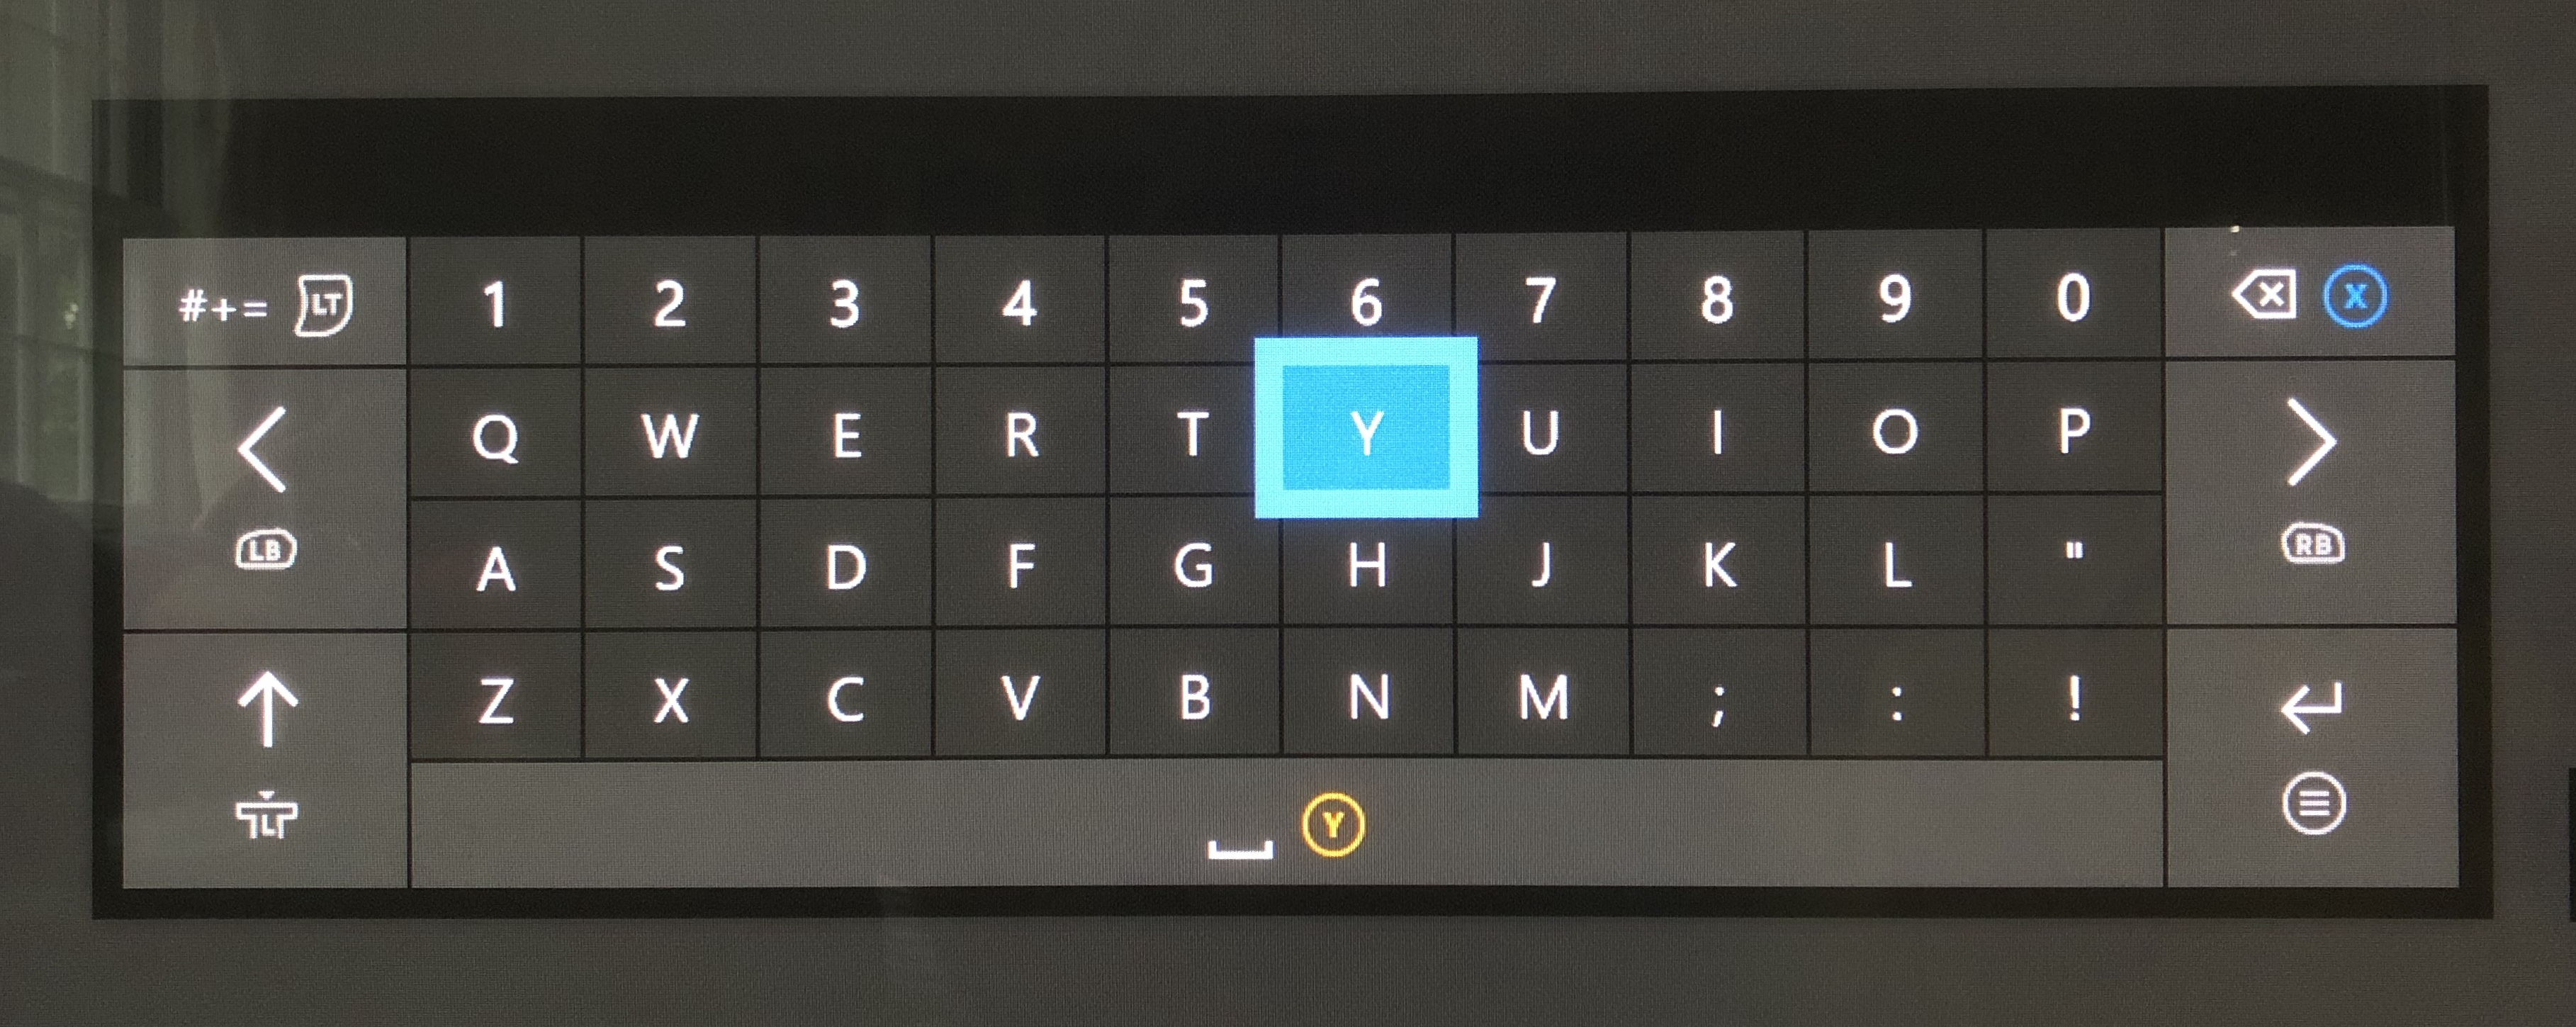
\includegraphics[width=9cm]{jdf-master/Figures/xbox-one-keyboard-photo.jpg}
	\caption{Photograph of the Xbox One onscreen keyboard}
	\label{fig:keyboard-photo}
\end{figure}

The first principle, which is immediately evident, is that of \textbf{Consistency}. The keyboard looks exactly like any other text entry keyboard, whether in real life i.e. a physical keyboard, or any other screen based virtual keyboard. It is therefore obvious to the casual observer what is expected - text entry. 

Related to this is the principle of \textbf{Mapping}. The user will be able to see the keyboard and correlate it to similar concepts on other platforms, or the physical world equivalent.

The next observation we can make is that the keyboard also adheres to the principle of \textbf{Perceptibility}. As can be seen in Figure \ref{fig:keyboard-photo}, the letter \textbf{\textit{Y}} is highlighted with a blue box and a bright blue border around that box. It is clear that this letter is currently selected. Moving any of the directional inputs on the controller will move the selection box to the next letter, in any of the 4 directions. Here, the directional inputs on the controller refer to the left and right thumbsticks and the cursor keypad.

The \textbf{Feedback} is also instant - as soon as a user moves the selection in any direction, the selection box immediately moves and lets the user know that the manipulation by hand of the controller inputs has had an action.

The final principle that we will touch on is \textbf{Discoverability}. It is obvious to the first time user that moving the thumbsticks moves the letters. It is also obvious what the user should do in case they make a mistake - the backspace icon is standard and next to it is placed the letter \textbf{\textit{X}} in a blue circle. This corresponds to the same button on the controller. In other words, the interface is informing you that the X button on the controller works as a backspace button. We see the same for the space bar at the bottom - the controller's \textbf{\textit{Y}} button activates the spacebar.

What about the other buttons? There are shapes marked with letters such as \textbf{LR, LB, RB}, something that looks like a table and something that looks like 3 lines in a circle? We cover them in the next subsection, on the negative attributes of the keyboard interface.

Finally, we observe that the Xbox One Virtual Keyboard follows the principle of \textbf{Simplicity}. There is nothing on screen, other than the keyboard, and the input field. Nothing to distract the user, allowing the user to focus on the task at hand.


\subsubsection{What doesn't work well and why?}
In the previous subsection we have said that \textit{The Xbox One Virtual Keyboard (keyboard) works perfectly well for any user who comes across the Xbox and has at least a modicum of knowledge about game controllers and how to manipulate thumbsticks}.

In other words, if you have not had any experience with a video game console controller with thumbsticks, you may not understand what to do when faced with an onscreen keyboard on the Xbox (however, to get till the keyboard, you would have had to use the controller, so this might be a moot point). The onscreen visuals do not clearly tell you to use the thumbsticks. We can say that the principle of \textbf{Discoverablity} is violated.

Secondly, even if you do understand that you have to use the controller thumbsticks to move the letter selector around, that doesn't mean that you will be able to achieve that. This requires hand-eye co-ordination quite different from other physical computer interfaces like a mouse or a touchscreen. It is not easy the first few times. In other words, it violates, or at least does not fully adhere to the principles of \textbf{Ease} and \textbf{Comfort}.

We discussed that the keyboard does tell you which letter buttons have additional functions on the keyboard, such as space and backspace. But there are other buttons there that do not make as much sense to the novice - for example the shift button is shown as something similar to a table - in actuality that is the cross section of the thumbstick, and the interface is telling you to press it axially. There are other buttons labelled LB, RB and LT. And they are inside funny shapes. A casual user would not know what they mean, one would have to read the Xbox One user manual for that (they refer to the buttons left bumber, right bumper and left trigger). Even someone who's used other console controllers may not realize what these buttons are, since they are specific to the Xbox. Therefore we can argue that \textbf{Discoverability} suffers here.

Finally, to manipulate the Xbox controller, one requires a certain dexterity of the hand. Older people with joint issues, younger children with small hands and differently abled persons with limited motor skills may not be able to use the controller to use the keyboard. This is a case of failing the principle of \textbf{Equity}. That said, this is not limited to the keyboard, this would follow the user everywhere on the console. And Microsoft, the manufacturer of the Xbox One, has a solution for the differently abled - the Xbox Adaptive Controller (\url{https://www.xbox.com/en-US/accessories/controllers/xbox-adaptive-controller}), which can be adapted in a myriad of ways for your levels of physical ability and dexterity.


\subsection{Conclusions}
The Xbox One Virtual Keyboard (keyboard) is a reasonably good interface, when seen against the major principles of design. It is easy to use, obvious to use, works with users of different skill levels and does not veer from consistency with other similar interfaces.

However, we believe that there is one additional principle - which was not included in chapter 2 - that applies here - and that is \textbf{Efficiency} (or alternatively \textbf{Effectiveness} - we can discuss the vocabulary).

The interface should lend itself to being an effective and efficient manner of input, where the user's intentions are converted to the desired effect in the computer with the least amount of effort. For example, in the least number of clicks or the least number of movements of the thumbsticks, the user should be able to enter any arbitrary text, limited only by their proficiency at the thumbstick.

We must concede here that an interface that tries to cater to advanced users, or provide a more complicated (albeit faster) way to achieve a task does not serve the less expert users of the platform. Therefore any redesign that takes away from ease of use and discoverability should be provided as an alternative to the existing simpler interface. By doing so, we would adhere to the principle of \textbf{Flexibility}. We shall discuss that in the next section.


\section{Interface Redesign}
\subsection{Overview of Redesign}
Our redesign of the Xbox One Virtual Keyboard will draw on the prior work done by \cite{eatsy_taplin_chechik_nelson_2002}, \cite{twostick_2007} and \cite{wilson_agrawala_2006}. Our design will use both thumbsticks to operate the on-screen keyboard, with the option for a circular menu of letters and also a split left/right keyboard where each half is operated by the respective thumbstick.

\subsection{Dual Circular Keyboard}
Our first design consists of a dual-circular keyboard. The high level features are as follows:
\begin{itemize}
    \item Keyboard is divided into left and right halves, corresponding to the left and right half of a QWERTY keyboard.
    \item The keys on the keyboard are exploded and arranged in a circular manner.
    \item The left side letters form the left circle with the letter Q on the top left (10:30 position) and the B key on the bottom right (4:30 position).
    \item The right side letters form the right circle with the letter P on the top middle right (1:00 position) and again the letter B on the bottom left (7:30) position.
    \item The letters are highlighted by the two thumbsticks, with the left thumbstick operating on the left circle and the right thumbstick operating on the right circle.
    \item Moving the thumbsticks highlights a letter on the circles, corresponding to the position the thumbstick is in. If the thumbstick is pointing to the top left, the top left letter on the circle is selected.
    \item The letter which is selected can be typed by clicking on the trigger associated with that side i.e. clicking the left trigger click types the letter selected by the left thumbstick.
    \item The default - center - position of the left thumbstick corresponds to the space bar.
    \item The default - center - position on the right thumbstick corresponds to the backspace button.
    \item Shift is activated by the shoulder buttons.
    \item Special symbols are activated by axially clicking the thumbsticks.
    \item The letter A (green) button is equivalent to ENTER.
    \item The letter B (red) button is equivalent to back or ESC.
\end{itemize}

An illustration of the dual circular keyboard can be seen in Figure \ref{fig:circular-keyboard}. Here we see the keyboard laid out in two circles. The letters T and K are highlighted because the left thumbstick is at the 1 o'clock position and the right thumbstick is on the 8 o'clock position. 

\begin{figure}[h]
	\centering
	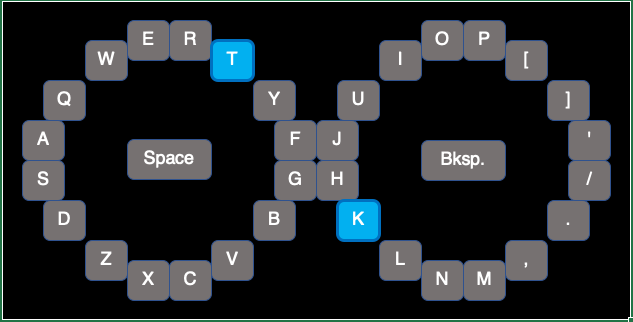
\includegraphics[width=9cm]{jdf-master/Figures/dual-circular-keyboard.png}
	\caption{Redesigned Keyboard - Dual Circular}
	\label{fig:circular-keyboard}
\end{figure}

The \textbf{key point} to note about the thumbsticks is that their relation to the on-screen keyboard is via \textit{\textbf{absolute positioning}}. If we were to move the left thumbstick from the 1 o'clock position to the 10 o'clock position, it would select the letter Q. This would be one movement of the thumbstick, but it would move across 4 letters on the circular keyboard. Thus, to move from any key to any key on the circle would require a single move of the thumbstick. The user would need to be able to control the angle of the thumbstick (here, we can refer to its polar co-ordinate representation, $\theta$) precisely.

If the user were to press the left trigger, it would send the keypress T and if the user were to press the right trigger, it would send the keypress K. We don't have to worry about the user pressing both triggers at the same time - the Xbox sensors work at a high frequency and can make out which one was pressed first and which one was pressed second, since it has to handle that level of detail in a game's controls.



\subsection{Dual Circular Concentric Keyboard}
We propose an additional performance enhancement for the \textit{Dual Circular} keyboard, which we call the \textit{Dual Circular Concentric} keyboard. An illustration of it can be seen in Figure \ref{fig:circular-concentric-keyboard}. Here, we add an additional set of keyboard buttons in a concentric circle inside the main circle. This contains the remainder of the keyboard - numbers and special symbols. 

\begin{figure}[h]
	\centering
	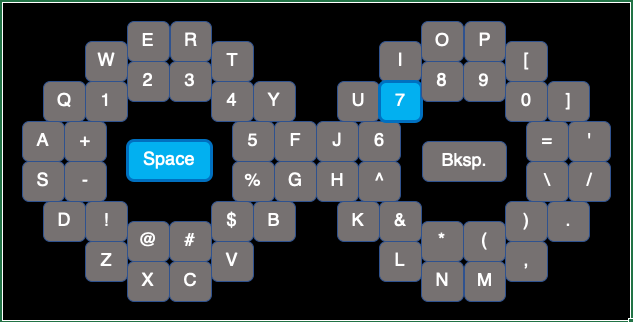
\includegraphics[width=9cm]{jdf-master/Figures/dual-circular-concentric-keyboard.png}
	\caption{Redesigned Keyboard - Dual Circular Concentric}
	\label{fig:circular-concentric-keyboard}
\end{figure}

While in the non-concentric dual circular design, we would have to click on the thumbstick to switch to the special character input, here we do not have to do that, and can select the special characters directly. The trade-off is that the user must be proficient in use of the thumbstick. It is not sufficient to think of just the angular position of the thumbstick, one would also have to have control over the amplitude of the thumbstick position (i.e. not just $\theta$ but also R)

Again, a move from any one letter on the keyboard to any other letter on the keyboard would be a single move of the thumbstick. In Figure \ref{fig:circular-concentric-keyboard} the left thumbstick is at rest in the center. To select the number 1, the user would move the thumbstick to the 10:30 position, but not entirely to the end of its travel. This would be one movement of the thumbstick. To then select V, the user would move the left thumbstick to the 5 o'clock position to the extreme end of its travel. This would also be a single movement of the thumbstick.

As before, clicking on the triggers would send the keypress of the selected letter.

The \textit{Dual Circular Concentric} approach could allow for even faster typing for the experienced gamer who has mastered control of the thumbstick, at the tradeoff of being difficult to use for everyone else.

\section{Interface Justification}
This interface redesign was done with the aim of increasing the efficiency of the interface (i.e. how quickly can a user achieve their aim) while not giving up too many of the advantages of the original design. The only exception to this is ease of use - this interface will not be as easy to use for a novice, it is geared towards experts/experienced gamers.

\subsection{What we Improved}
The key improvement that this interface tries to bring about is on the principle of \textbf{Efficiency}. The idea is that a user will be able to use this input method to type more quickly than with the standard QWERTY onscreen keyboard.

The reasoning behind this is as explained in the previous section - to move from any one character to another character on the keyboard requires exactly one move of a thumbstick. In contrast, with the existing keyboard, it can take as many as 7 individual actions to go from one letter to the next. 

For example, if one wanted to type the two letters \textbf{CI}, one would use either thumbstick to make the following movements in the QWERTY keyboard. Starting at the letter C, we would press A, right, right, right, right, right, up, up, A, for a total of 9 individual actions.

For the same characters on the dual circular keyboard or the concentric dual circular keyboards, we would make the following movements: Starting at rest, press: Left thumbstick down, left trigger, right thumbstick upper left, right trigger, for a total of 4 individual actions. 

The key point is that for any two combinations of keys that are on screen at a given time, the circular keyboards (concentric or not) would require exactly 4 actions every time. 

If we were to extend this to all characters, then the QWERTY keyboard would take up to 11 keypresses (the two additional keypresses to move to symbol mode, then back to regular mode), the dual concentric keyboard would take at most 6 keypresses (press axially while moving to select from the symbols character set) and the concentric dual circular keyboard \textit{would still take only 4 actions to access any character on the keyboard.}

\subsection{What we Changed}
To the casual user, it seems that we have lost the principle of  \textbf{Consistency}. The keyboard no longer looks like other keyboards. It does still contain letters/buttons, and has QWERTY shown on screen, but thats where the comparison stops.

To an expert user i.e. committed gamer, the keyboard looks very similar to other such circular selection menus in video games that the user would have played on the very same console. We use the example of the console game Red Dead Redemption 2, a re-imagining of the classic cowboy western (\cite{schwartz_2018}) where the player selects their in-game weapon by using a selection wheel, as can be seen in Figure \ref{fig:weapon-wheel}. Therefore we do maintain \textbf{Consistency}, but now we are consistent to a different standard.

\begin{figure}[h]
	\centering
	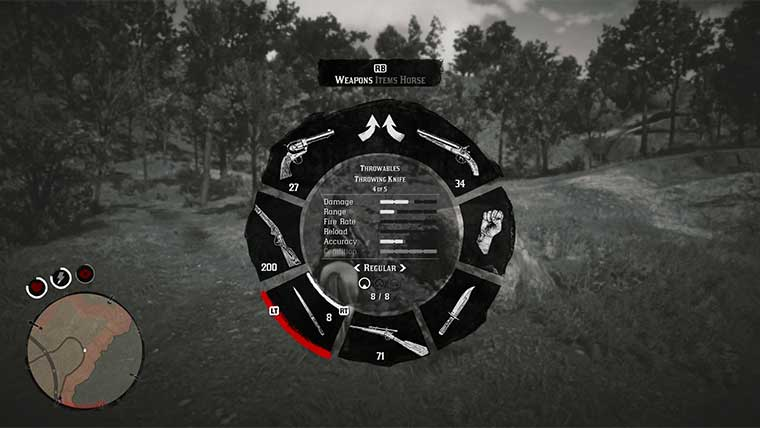
\includegraphics[width=9cm]{jdf-master/Figures/weapon-wheel-red-dead-redemption-2.jpg}
	\caption{Weapon Wheel, Red Dead Redemption}
	\label{fig:weapon-wheel}
\end{figure}


Related to this is the principle of \textbf{Mapping}. The expert gamer will be able to map the circular keyboard to other similar selection wheels on the console.




\subsection{What we Kept}

We maintain that the circular keyboard also adheres to the principle of \textbf{Perceptibility}. As can be seen in Figure \ref{fig:circular-keyboard}, the letters \textbf{\textit{T \& K}} are highlighted with a blue box. It is clear that these letter are currently selected. 

The \textbf{Feedback} is also instant - as soon as a user moves the selection in any direction, the selection box immediately moves and lets the user know that the manipulation by hand of the controller inputs has had an action, just like in the regular onscreen QWERTY keyboard.

The final principle that we will touch on is \textbf{Discoverability}. It is obvious to the first time user that moving the thumbsticks moves the letters. It is also obvious what the user should do in case they make a mistake - the backspace button is prominent.

While we have not shown in in our diagram, there is nothing preventing us from showing what functions the other buttons have, such as the Left Trigger, Right Trigger, Left Bumper, Right Bumper, A and B.

Finally, maintain the principle of \textbf{Simplicity}. There is nothing on screen, other than the keyboard, and the input field. Nothing to distract the user, allowing the user to focus on the task at hand.

The principle of \textbf{Discoverablity} remains unchanged as we switch from the QWERTY keyboard to the dual-circular keyboards. They make it equally difficult or equally easy to discover the functionality of the various input controls on the controller to control the keyboard.


\subsection{What we Lost}
What we lost almost entirely is the principle of \textbf{Ease}. This is not an easy keyboard to use. The novice user will not be able to use it. Similarly, the keyboard will not be helpful to users of different levels of ability, and therefore the principle of \textbf{Equity} is also violated. That said, it remains to be seen how users of the Xbox Adaptive Controller find this keyboard.

\subsection{What we can Add}
The current keyboard for the Xbox is fixed - it is not configurable.

The Dual Circular Keyboard and the Dual Circular Concentric Keyboard could be added as options in the Xbox setting, wherein a user could go and select which of the three keyboards they would like to use on the Xbox. In this way, the default keyboard could remain the onscreen QWERTY, while still giving the user the option to upgrade functionality to Dual Circular or Dual Circular Concentric. In this way, we gain the principle of \textbf{Flexibility}.

Among the possible options I would also recommend we add the Dual Stick QWERTY keyboard (see Figure \ref{fig:dual-stick-qwerty}) as described in \textit{"Text entry using a dual joystick game controller"} (\cite{wilson_agrawala_2006}). This keyboard brings in some of the benefits of a dual-stick input, while maintaining \textbf{Consistency} and similar levels of \textbf{Ease} as a standard one-stick QWERTY keyboard.

\begin{figure}[h]
	\centering
	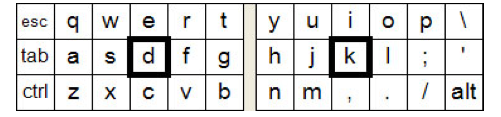
\includegraphics[width=9cm]{jdf-master/Figures/dual-stick-keyboard.png}
	\caption{Dual Stick QWERTY onscreen keyboard - the left and right highlighted characters indicate the charactor to be entered upon hitting the left and right triggers on the controller, respectively.}
	\label{fig:dual-stick-qwerty}
\end{figure}



\section{Evaluation Plan}
We shall evaluate the new keyboard via an empirical evaluation. Our objective is to determine if the new design does actually help experienced gamers type more efficiently than the standard keyboard.

\subsection{Control Group}

\subsection{Experimental Group}

\subsection{Null Hypothesis}

\subsection{Alternative Hypothesis}

\subsection{Variables}

\subsection{Statistical Analysis}

\section{References}

\printbibliography[heading=none]


\end{document}